\pdfoutput=1
\documentclass[aspectratio=169,10pt]{beamer}
\pdfmapfile{+cm.map}
\pdfmapfile{+cmextra.map}
\pdfmapfile{+symbols.map}
\usepackage{amsmath,amssymb}
\usepackage{tikz}
\usepackage{pgfplots}
\pgfplotsset{compat=1.18}
\definecolor{ink}{HTML}{142D42}
\definecolor{teal}{HTML}{007C83}
\definecolor{light}{HTML}{F0F6F6}
\setbeamercolor{normal text}{fg=ink,bg=white}
\setbeamercolor{frametitle}{fg=ink,bg=white}
\setbeamercolor{structure}{fg=teal}
\setbeamercolor{block title}{fg=white,bg=teal}
\setbeamercolor{block body}{fg=ink,bg=light}
\setbeamertemplate{navigation symbols}{}
\setbeamertemplate{footline}{\leavevmode\hbox{\hspace{0.5cm}\scriptsize Stochastic kinetics\hfill\insertframenumber\hspace{0.5cm}}\vspace{0.2cm}}
\setbeamertemplate{itemize items}[circle]
\setbeamersize{text margin left=0.7cm,text margin right=0.7cm}
\title{Stochastic kinetics}
\subtitle{From Brownian trajectories to Fokker--Planck and first passage}
\author{Giuseppe Stefano Basile}
\institute{Hands-on lesson}
\date{}
\newcommand{\E}{\mathbb{E}}
\newcommand{\dd}{\mathrm{d}}
\begin{document}
\begin{frame}\titlepage\end{frame}
\begin{frame}{The question behind this lesson}
\begin{block}{A molecular transition}Given a free-energy landscape and a diffusion coefficient, how long does it take to reach a product state?\end{block}
\begin{itemize}\item Start with individual noisy trajectories.\item Derive an equation for their probability density.\item Predict a mean first-passage time and test it numerically.\end{itemize}
\end{frame}
\begin{frame}{Road map and learning objectives}
\begin{enumerate}\item Probability, ensembles and Brownian motion.\item Langevin dynamics and the Fokker--Planck equation.\item First passage, numerical comparisons and molecular limits.\end{enumerate}
\vspace{0.4cm}\textbf{Afterwards:} derive the main equations, run the examples and identify when assumptions may fail. The foundations require 60--90 minutes of preparation or additional class time.
\end{frame}
\begin{frame}{A probability density is not a probability}
A random variable $X$ has density $p(x)$ when
\[\Pr(c<X<d)=\int_c^d p(x)\,\dd x,\qquad \int p(x)\,\dd x=1.\]
\begin{itemize}\item $p(x)$ has units of $1/x$. The area under it is a probability.\item The mean $\E[X]$ locates the ensemble average.\item The variance $\mathrm{Var}(X)=\E[(X-\E X)^2]$ measures spread.\end{itemize}
\end{frame}
\begin{frame}{Samples, uncertainty and correlation}
For $N$ independent samples, estimate the mean and its standard error by
\[\bar X=\frac{1}{N}\sum_{i=1}^{N}X_i,\qquad \mathrm{SE}(\bar X)\approx \frac{s}{\sqrt N}.\]
\begin{itemize}\item Standard deviation describes variation between outcomes.\item Standard error describes uncertainty in the estimated mean.\item Consecutive trajectory frames are generally correlated.\end{itemize}
\begin{block}{Try it}Compare histograms for $N=100$ and $N=10\,000$ in the foundations notebook.\end{block}
\end{frame}
\begin{frame}{Process, path and Markov property}
\begin{itemize}\item A process $\{X_t\}_{t\geq0}$ is a family of random variables.\item A trajectory is one realization. A density describes an ensemble.\item Markov property: given the present state, the future is independent of its past.\end{itemize}
\vspace{0.3cm}For a molecular coordinate, omitted degrees of freedom can carry memory. Markovianity must be assessed for the chosen state.
\end{frame}

\begin{frame}{Transition densities and the Markov assumption}
For a time-homogeneous Markov process with transition density
$p_t(y\mid x)$, conditioning on the intermediate state gives
\[
p_{t+s}(y\mid x)=\int p_t(y\mid z)\,p_s(z\mid x)\,\dd z.
\]
\begin{itemize}
\item The integral sums all intermediate positions $z$.
\item This Chapman--Kolmogorov relation is a model check at chosen lag times.
\item An equilibrium density alone does not specify $p_t(y\mid x)$.
\end{itemize}
\end{frame}
\begin{frame}{Our investigation and route through the lesson}
\begin{block}{One experiment}
A particle starts in the left well. How long until it first reaches the right well?
\end{block}
\begin{enumerate}
\item Predict and simulate trajectories, then inspect the evolving density.
\item Define the first-passage event and compute its mean from paths.
\item Derive a prediction from the backward equation and compare methods.
\item Vary $D$, barrier height and target. Check statistical and numerical errors.
\end{enumerate}
\end{frame}
\begin{frame}{Brownian motion: the noise model}
Standard Brownian motion $W_t$ has independent increments
\[\Delta W=W_{t+\Delta t}-W_t\sim\mathcal N(0,\Delta t).\]
Hence $\Delta W=\sqrt{\Delta t}\,\xi$ with $\xi\sim\mathcal N(0,1)$.
\begin{itemize}\item Paths are continuous but almost surely nowhere differentiable.\item $\dot W$ is formal white-noise notation.\item The variance of an increment is $\Delta t$.\end{itemize}
\end{frame}
\begin{frame}{Free diffusion}
\[\dd X_t=\sqrt{2D}\,\dd W_t,\qquad X_0=x_0.\]
\[\E[X_t]=x_0,\qquad \mathrm{Var}(X_t)=2Dt.\]
A single path fluctuates. The ensemble variance grows linearly in time.
\begin{block}{Units and prediction}$[D]=\mathrm{length}^2/\mathrm{time}$. What happens if $D$ doubles?\end{block}
\end{frame}
\begin{frame}{Hands-on 1: trajectories and ensembles}
\textbf{Open:} \texttt{notebooks/00\_foundations.ipynb}, section 2.
\[X_{n+1}=X_n+\sqrt{2D\Delta t}\,\xi_n,\qquad \xi_n\sim\mathcal N(0,1).\]
\begin{enumerate}\item Plot several trajectories and the ensemble variance.\item Compare the variance with $2Dt$.\item Replace $\sqrt{\Delta t}$ with $\Delta t$. What fails as $\Delta t\to0$?\end{enumerate}
\end{frame}
\begin{frame}{A particle in a thermal environment}
An underdamped Langevin model reads
\[\dd x=v\,\dd t,\quad m\dd v=[-U'(x)-\zeta v]\dd t+\sqrt{2\zeta k_BT}\,\dd W_t.\]
\begin{itemize}\item $U$: potential energy, $\zeta$: friction, $T$: temperature.\item Friction and fluctuations satisfy a fluctuation--dissipation relation.\item If velocity relaxes rapidly, an overdamped position model may apply.\end{itemize}
\end{frame}
\begin{frame}{Overdamped Langevin equation}
For constant mobility $\mu=1/\zeta$, define $D=\mu k_BT$ and $\beta=(k_BT)^{-1}$. Then
\[\boxed{\dd X_t=-D\beta F'(X_t)\,\dd t+\sqrt{2D}\,\dd W_t.}\]
The first term is drift. The second describes diffusion.
\begin{block}{Modeling assumption}Using a free energy $F$ and Markovian diffusion for a molecular collective variable is an additional approximation.\end{block}
\end{frame}
\begin{frame}{Euler--Maruyama: simulate the model}
\[X_{n+1}=X_n-D\beta F'(X_n)\Delta t+\sqrt{2D\Delta t}\,\xi_n.\]
\begin{itemize}\item Evaluate coefficients at the start of each step: It\^o convention.\item Draw independent standard normal $\xi_n$ values.\item Discretization introduces error: repeat at smaller $\Delta t$.\end{itemize}
A finite ensemble also produces sampling uncertainty. These are distinct errors.
\end{frame}
\begin{frame}{Exactly solvable check: harmonic confinement}
Take $F(x)=\tfrac12\kappa x^2$ and $\lambda=D\beta\kappa$. For fixed $X_0=x_0$,
\[\E[X_t]=x_0e^{-\lambda t},\quad \mathrm{Var}(X_t)=\frac{D}{\lambda}(1-e^{-2\lambda t}).\]
\begin{itemize}\item At long times, $\mathrm{Var}(X)=1/(\beta\kappa)$.\item At fixed $F$ and $T$, $D$ changes relaxation time $1/\lambda$.\end{itemize}
\textbf{Notebook:} compare simulated moments to these exact curves.
\end{frame}
\begin{frame}{From an SDE to short-time conditional moments}
For $\dd X_t=a(X_t)\dd t+\sqrt{2D(X_t)}\dd W_t$, with smooth coefficients and $X_t=x$,
\[\E[\Delta X\mid x]=a(x)\Delta t+o(\Delta t),\quad
\E[(\Delta X)^2\mid x]=2D(x)\Delta t+o(\Delta t).\]
\begin{itemize}
\item Drift is the local first conditional moment per unit time.
\item Diffusion is half the local second conditional moment per unit time.
\item These limits assume an It\^o diffusion at sufficiently short times.
\end{itemize}
\end{frame}
\begin{frame}{Why It\^o calculus differs from ordinary calculus}
For $\dd X=a(X)\dd t+\sqrt{2D(X)}\dd W$ and smooth $f$,
\[\Delta f\approx f'(X)\Delta X+\tfrac12 f''(X)(\Delta X)^2.\]
Since $(\Delta W)^2$ contributes at order $\Delta t$, the quadratic term survives:
\[\boxed{\dd f=[af'+Df'']\dd t+\sqrt{2D}f'\dd W.}\]
Assume the regularity and integrability required to take expectations.
\end{frame}
\begin{frame}{It\^o formula: from increments to the generator}
For $\Delta X=a\Delta t+\sqrt{2D}\Delta W+o(\sqrt{\Delta t})$, expand
\[\E[\Delta f\mid X_t=x]=f'(x)\E[\Delta X\mid x]+\tfrac12 f''(x)\E[(\Delta X)^2\mid x]+o(\Delta t).\]
Dividing by $\Delta t$ and taking the limit gives
\[\lim_{\Delta t\to0}\frac{\E_x[f(X_{\Delta t})]-f(x)}{\Delta t}
=a(x)f'(x)+D(x)f''(x)=\mathcal Lf(x).\]
The finite-variation and quadratic-variation terms both contribute.
\end{frame}
\begin{frame}{Backward generator and forward density equation}
Define the backward generator acting on an observable $f$:
\[\mathcal Lf=af'+Df'',\qquad \frac{\dd}{\dd t}\E[f(X_t)]=\E[\mathcal Lf(X_t)].\]
Write the expectation as $\int f p\,\dd x$ and integrate by parts:
\[\boxed{\partial_t p=-\partial_x(ap)+\partial_x^2(Dp).}\]
\textbf{Forward:} evolve densities. \quad \textbf{Backward:} act on functions of the starting point.
\end{frame}


\begin{frame}{Forward equation: the adjoint calculation}
Assume smooth functions and boundary conditions cancelling the boundary terms. With $\mathcal L f=af'+Df''$,
\[
\int f\,\partial_t p\,\dd x
=\int (af'+Df'')p\,\dd x
=\int f\,[-(ap)'+(Dp)'']\,\dd x.
\]
As this holds for suitable test functions $f$,
\[\partial_t p=\mathcal L^*p=-(ap)'+(Dp)''.\]
\textbf{Boundary terms matter:} reflecting and absorbing boundaries define different operator domains and different physical experiments.
\end{frame}
\begin{frame}{Boundary terms: forward and backward conditions}
On $[a,b]$, two integrations by parts give
\[\int_a^b (\mathcal Lf)p\,\dd x-\int_a^b f(\mathcal L^*p)\,\dd x
=\big[fJ+Dp f'\big]_{a}^{b}.\]
For a reflecting left wall, $J(a)=0$ and backward observables satisfy $f'(a)=0$. For a regular absorbing right wall, the killed density satisfies $p(b)=0$ and the backward observable satisfies $f(b)=0$.
\vspace{0.2cm}
These boundary conditions cancel the corresponding boundary terms.
\end{frame}
\begin{frame}{Probability current and equilibrium}
\[\partial_t p=-\partial_xJ,\qquad J=ap-\partial_x(Dp).\]
For constant $D$, with $a=-D\beta F'$,
\[J=-D(\beta F'p+\partial_xp).\]
A normalizable zero-current equilibrium is $p_{\mathrm{eq}}(x)=Z^{-1}e^{-\beta F(x)}$.
\end{frame}

\begin{frame}{Position-dependent diffusion: the It\^o drift}
For $\dd X=a(X)\dd t+\sqrt{2D(X)}\,\dd W$, the current is
\[J=a p-\partial_x(Dp).\]
To obtain $p_{\rm eq}\propto e^{-\beta F}$ with zero current, choose
\[\boxed{a(x)=D'(x)-D(x)\beta F'(x).}\]
Then $\partial_t p=\partial_x[D e^{-\beta F}\partial_x(e^{\beta F}p)]$.
\begin{itemize}
\item The $D'$ term is required for this It\^o representation.
\item Other stochastic conventions require a transformed drift.
\end{itemize}
\end{frame}
\begin{frame}{Hands-on 2: a double-well free energy}
\begin{columns}
\column{0.46\textwidth}
\[F(x)=H(x^2-1)^2.\]
Minima: $x=\pm1$.\\
Barrier: $F(0)-F(\pm1)=H$.\\[0.3cm]
Simulate a trajectory and compare its histogram with $e^{-\beta F}/Z$.
\column{0.52\textwidth}
\begin{tikzpicture}\begin{axis}[width=\linewidth,height=5cm,axis lines=left,xlabel={$x$},ylabel={$F(x)$},domain=-1.5:1.5,samples=100,ymin=0,ymax=4.3,xtick={-1,0,1}]
\addplot[teal,very thick]{2*(x*x-1)^2};
\end{axis}\end{tikzpicture}
\end{columns}
\end{frame}
\begin{frame}{Ensemble density: trajectories and Fokker--Planck}
\begin{center}
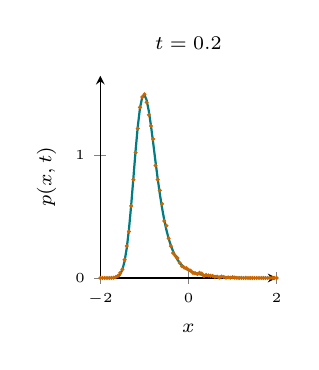
\begin{tikzpicture}\begin{axis}[width=.315\textwidth,height=4.15cm,axis lines=left,xmin=-2,xmax=2,ymin=0,ymax=1.65,xtick={-2,0,2},ytick={0,1},title={$t=0.2$},xlabel={$x$},ylabel={$p(x,t)$},title style={font=\scriptsize},tick label style={font=\tiny},label style={font=\scriptsize}]
\addplot[teal,thick] coordinates {(-2.000,0.0000) (-1.950,0.0000) (-1.900,0.0000) (-1.850,0.0000) (-1.800,0.0001) (-1.750,0.0003) (-1.700,0.0012) (-1.650,0.0042) (-1.600,0.0121) (-1.550,0.0307) (-1.500,0.0687) (-1.450,0.1372) (-1.400,0.2464) (-1.350,0.4010) (-1.300,0.5966) (-1.250,0.8179) (-1.200,1.0409) (-1.150,1.2387) (-1.100,1.3881) (-1.050,1.4743) (-1.000,1.4936) (-0.950,1.4518) (-0.900,1.3616) (-0.850,1.2386) (-0.800,1.0982) (-0.750,0.9533) (-0.700,0.8136) (-0.650,0.6853) (-0.600,0.5715) (-0.550,0.4734) (-0.500,0.3905) (-0.450,0.3215) (-0.400,0.2647) (-0.350,0.2183) (-0.300,0.1805) (-0.250,0.1498) (-0.200,0.1250) (-0.150,0.1047) (-0.100,0.0883) (-0.050,0.0748) (0.000,0.0638) (0.050,0.0547) (0.100,0.0471) (0.150,0.0409) (0.200,0.0356) (0.250,0.0311) (0.300,0.0273) (0.350,0.0241) (0.400,0.0213) (0.450,0.0189) (0.500,0.0168) (0.550,0.0149) (0.600,0.0133) (0.650,0.0118) (0.700,0.0104) (0.750,0.0092) (0.800,0.0080) (0.850,0.0069) (0.900,0.0059) (0.950,0.0050) (1.000,0.0041) (1.050,0.0033) (1.100,0.0025) (1.150,0.0019) (1.200,0.0013) (1.250,0.0009) (1.300,0.0006) (1.350,0.0003) (1.400,0.0002) (1.450,0.0001) (1.500,0.0000) (1.550,0.0000) (1.600,0.0000) (1.650,0.0000) (1.700,0.0000) (1.750,0.0000) (1.800,0.0000) (1.850,0.0000) (1.900,0.0000) (1.950,0.0000) (2.000,0.0000)};
\addplot[orange!80!black,only marks,mark=*,mark size=.5pt] coordinates {(-2.000,0.0000) (-1.950,0.0000) (-1.900,0.0000) (-1.850,0.0000) (-1.800,0.0000) (-1.750,0.0011) (-1.700,0.0022) (-1.650,0.0078) (-1.600,0.0178) (-1.550,0.0411) (-1.500,0.0711) (-1.450,0.1489) (-1.400,0.2611) (-1.350,0.3800) (-1.300,0.5878) (-1.250,0.8022) (-1.200,1.0233) (-1.150,1.2200) (-1.100,1.3922) (-1.050,1.4767) (-1.000,1.4989) (-0.950,1.4322) (-0.900,1.3311) (-0.850,1.2400) (-0.800,1.1333) (-0.750,0.9178) (-0.700,0.8033) (-0.650,0.7144) (-0.600,0.6044) (-0.550,0.4644) (-0.500,0.4267) (-0.450,0.3233) (-0.400,0.2600) (-0.350,0.2033) (-0.300,0.1811) (-0.250,0.1633) (-0.200,0.1233) (-0.150,0.0967) (-0.100,0.0844) (-0.050,0.0800) (0.000,0.0678) (0.050,0.0600) (0.100,0.0411) (0.150,0.0389) (0.200,0.0322) (0.250,0.0433) (0.300,0.0367) (0.350,0.0167) (0.400,0.0244) (0.450,0.0211) (0.500,0.0178) (0.550,0.0167) (0.600,0.0100) (0.650,0.0111) (0.700,0.0033) (0.750,0.0122) (0.800,0.0078) (0.850,0.0022) (0.900,0.0056) (0.950,0.0022) (1.000,0.0067) (1.050,0.0033) (1.100,0.0011) (1.150,0.0000) (1.200,0.0011) (1.250,0.0000) (1.300,0.0011) (1.350,0.0000) (1.400,0.0000) (1.450,0.0000) (1.500,0.0000) (1.550,0.0000) (1.600,0.0000) (1.650,0.0000) (1.700,0.0000) (1.750,0.0000) (1.800,0.0000) (1.850,0.0000) (1.900,0.0000) (1.950,0.0000) (2.000,0.0000)};
\end{axis}\end{tikzpicture}
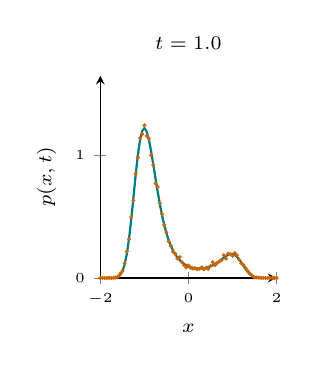
\begin{tikzpicture}\begin{axis}[width=.315\textwidth,height=4.15cm,axis lines=left,xmin=-2,xmax=2,ymin=0,ymax=1.65,xtick={-2,0,2},ytick={0,1},title={$t=1.0$},xlabel={$x$},ylabel={$p(x,t)$},title style={font=\scriptsize},tick label style={font=\tiny},label style={font=\scriptsize}]
\addplot[teal,thick] coordinates {(-2.000,0.0000) (-1.950,0.0000) (-1.900,0.0000) (-1.850,0.0000) (-1.800,0.0001) (-1.750,0.0003) (-1.700,0.0010) (-1.650,0.0033) (-1.600,0.0095) (-1.550,0.0242) (-1.500,0.0544) (-1.450,0.1088) (-1.400,0.1958) (-1.350,0.3194) (-1.300,0.4764) (-1.250,0.6550) (-1.200,0.8363) (-1.150,0.9990) (-1.100,1.1243) (-1.050,1.2000) (-1.000,1.2225) (-0.950,1.1960) (-0.900,1.1301) (-0.850,1.0369) (-0.800,0.9286) (-0.750,0.8154) (-0.700,0.7052) (-0.650,0.6032) (-0.600,0.5120) (-0.550,0.4328) (-0.500,0.3653) (-0.450,0.3088) (-0.400,0.2620) (-0.350,0.2235) (-0.300,0.1920) (-0.250,0.1664) (-0.200,0.1456) (-0.150,0.1288) (-0.100,0.1153) (-0.050,0.1044) (0.000,0.0959) (0.050,0.0892) (0.100,0.0843) (0.150,0.0808) (0.200,0.0787) (0.250,0.0779) (0.300,0.0784) (0.350,0.0803) (0.400,0.0836) (0.450,0.0884) (0.500,0.0948) (0.550,0.1029) (0.600,0.1128) (0.650,0.1243) (0.700,0.1373) (0.750,0.1512) (0.800,0.1653) (0.850,0.1783) (0.900,0.1887) (0.950,0.1949) (1.000,0.1951) (1.050,0.1882) (1.100,0.1737) (1.150,0.1524) (1.200,0.1262) (1.250,0.0980) (1.300,0.0707) (1.350,0.0471) (1.400,0.0287) (1.450,0.0159) (1.500,0.0079) (1.550,0.0035) (1.600,0.0014) (1.650,0.0005) (1.700,0.0001) (1.750,0.0000) (1.800,0.0000) (1.850,0.0000) (1.900,0.0000) (1.950,0.0000) (2.000,0.0000)};
\addplot[orange!80!black,only marks,mark=*,mark size=.5pt] coordinates {(-2.000,0.0000) (-1.950,0.0000) (-1.900,0.0000) (-1.850,0.0000) (-1.800,0.0011) (-1.750,0.0000) (-1.700,0.0011) (-1.650,0.0033) (-1.600,0.0111) (-1.550,0.0333) (-1.500,0.0567) (-1.450,0.1211) (-1.400,0.2167) (-1.350,0.3167) (-1.300,0.4978) (-1.250,0.6333) (-1.200,0.8489) (-1.150,0.9833) (-1.100,1.1422) (-1.050,1.1756) (-1.000,1.2456) (-0.950,1.1600) (-0.900,1.1378) (-0.850,1.0022) (-0.800,0.9222) (-0.750,0.7711) (-0.700,0.7422) (-0.650,0.6089) (-0.600,0.5222) (-0.550,0.4333) (-0.500,0.3722) (-0.450,0.2989) (-0.400,0.2611) (-0.350,0.2133) (-0.300,0.1978) (-0.250,0.1600) (-0.200,0.1711) (-0.150,0.1300) (-0.100,0.1056) (-0.050,0.0856) (0.000,0.1011) (0.050,0.0833) (0.100,0.0767) (0.150,0.0800) (0.200,0.0711) (0.250,0.0756) (0.300,0.0878) (0.350,0.0700) (0.400,0.0822) (0.450,0.0733) (0.500,0.0978) (0.550,0.1289) (0.600,0.1044) (0.650,0.1222) (0.700,0.1356) (0.750,0.1444) (0.800,0.1856) (0.850,0.1578) (0.900,0.1989) (0.950,0.1956) (1.000,0.1811) (1.050,0.2044) (1.100,0.1856) (1.150,0.1500) (1.200,0.1189) (1.250,0.1056) (1.300,0.0789) (1.350,0.0544) (1.400,0.0333) (1.450,0.0200) (1.500,0.0044) (1.550,0.0044) (1.600,0.0022) (1.650,0.0000) (1.700,0.0011) (1.750,0.0000) (1.800,0.0000) (1.850,0.0000) (1.900,0.0000) (1.950,0.0000) (2.000,0.0000)};
\end{axis}\end{tikzpicture}
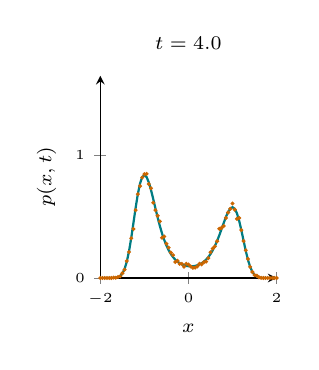
\begin{tikzpicture}\begin{axis}[width=.315\textwidth,height=4.15cm,axis lines=left,xmin=-2,xmax=2,ymin=0,ymax=1.65,xtick={-2,0,2},ytick={0,1},title={$t=4.0$},xlabel={$x$},ylabel={$p(x,t)$},title style={font=\scriptsize},tick label style={font=\tiny},label style={font=\scriptsize}]
\addplot[teal,thick] coordinates {(-2.000,0.0000) (-1.950,0.0000) (-1.900,0.0000) (-1.850,0.0000) (-1.800,0.0000) (-1.750,0.0002) (-1.700,0.0007) (-1.650,0.0022) (-1.600,0.0065) (-1.550,0.0165) (-1.500,0.0371) (-1.450,0.0742) (-1.400,0.1335) (-1.350,0.2179) (-1.300,0.3253) (-1.250,0.4475) (-1.200,0.5718) (-1.150,0.6837) (-1.100,0.7702) (-1.050,0.8232) (-1.000,0.8399) (-0.950,0.8232) (-0.900,0.7795) (-0.850,0.7172) (-0.800,0.6444) (-0.750,0.5681) (-0.700,0.4938) (-0.650,0.4249) (-0.600,0.3634) (-0.550,0.3100) (-0.500,0.2646) (-0.450,0.2268) (-0.400,0.1956) (-0.350,0.1702) (-0.300,0.1498) (-0.250,0.1335) (-0.200,0.1207) (-0.150,0.1110) (-0.100,0.1038) (-0.050,0.0988) (0.000,0.0959) (0.050,0.0949) (0.100,0.0959) (0.150,0.0987) (0.200,0.1037) (0.250,0.1109) (0.300,0.1208) (0.350,0.1337) (0.400,0.1501) (0.450,0.1705) (0.500,0.1956) (0.550,0.2258) (0.600,0.2615) (0.650,0.3026) (0.700,0.3488) (0.750,0.3986) (0.800,0.4495) (0.850,0.4980) (0.900,0.5392) (0.950,0.5676) (1.000,0.5776) (1.050,0.5649) (1.100,0.5276) (1.150,0.4676) (1.200,0.3906) (1.250,0.3053) (1.300,0.2217) (1.350,0.1484) (1.400,0.0909) (1.450,0.0505) (1.500,0.0252) (1.550,0.0112) (1.600,0.0044) (1.650,0.0015) (1.700,0.0005) (1.750,0.0001) (1.800,0.0000) (1.850,0.0000) (1.900,0.0000) (1.950,0.0000) (2.000,0.0000)};
\addplot[orange!80!black,only marks,mark=*,mark size=.5pt] coordinates {(-2.000,0.0000) (-1.950,0.0000) (-1.900,0.0000) (-1.850,0.0000) (-1.800,0.0000) (-1.750,0.0000) (-1.700,0.0033) (-1.650,0.0022) (-1.600,0.0078) (-1.550,0.0133) (-1.500,0.0389) (-1.450,0.0678) (-1.400,0.1389) (-1.350,0.2122) (-1.300,0.3244) (-1.250,0.4000) (-1.200,0.5533) (-1.150,0.6844) (-1.100,0.7500) (-1.050,0.8200) (-1.000,0.8467) (-0.950,0.8500) (-0.900,0.7667) (-0.850,0.7322) (-0.800,0.6144) (-0.750,0.5533) (-0.700,0.5078) (-0.650,0.4622) (-0.600,0.3289) (-0.550,0.3389) (-0.500,0.2800) (-0.450,0.2478) (-0.400,0.2078) (-0.350,0.1867) (-0.300,0.1300) (-0.250,0.1400) (-0.200,0.1156) (-0.150,0.1156) (-0.100,0.0922) (-0.050,0.1167) (0.000,0.1100) (0.050,0.0944) (0.100,0.0833) (0.150,0.0844) (0.200,0.0944) (0.250,0.1156) (0.300,0.1111) (0.350,0.1289) (0.400,0.1333) (0.450,0.1622) (0.500,0.2100) (0.550,0.2400) (0.600,0.2578) (0.650,0.3000) (0.700,0.4011) (0.750,0.4089) (0.800,0.4244) (0.850,0.4900) (0.900,0.5344) (0.950,0.5644) (1.000,0.6078) (1.050,0.5578) (1.100,0.4822) (1.150,0.4900) (1.200,0.3911) (1.250,0.3011) (1.300,0.2267) (1.350,0.1556) (1.400,0.0911) (1.450,0.0489) (1.500,0.0233) (1.550,0.0189) (1.600,0.0056) (1.650,0.0011) (1.700,0.0000) (1.750,0.0000) (1.800,0.0000) (1.850,0.0000) (1.900,0.0000) (1.950,0.0000) (2.000,0.0000)};
\end{axis}\end{tikzpicture}
\end{center}
\vspace{-0.2cm}\scriptsize
\textcolor{teal}{Line}: detailed-balance grid generator. \textcolor{orange!80!black}{Dots}: independent Euler--Maruyama paths. $F=2(x^2-1)^2$, $D=\beta=1$, $x_0=-1$; both ends reflect at $\pm2$.
\end{frame}
\begin{frame}{Same equilibrium, different kinetics}
At fixed $F$ and $T$, replace $D$ by $cD$:
\begin{itemize}\item $p_{\mathrm{eq}}$ is unchanged.\item The generator is multiplied by $c$.\item First-passage times scale by $1/c$.\end{itemize}
\begin{block}{Discuss}What does an equilibrium free-energy surface tell us? What information is still needed for a time scale?\end{block}
\end{frame}
\begin{frame}{First-passage time: define the experiment}
Start at $x_0$, reflect at $a$, and absorb at target $b$:
\[\tau_b=\inf\{t\geq0:X_t\geq b\},\qquad T(x_0)=\E_{x_0}[\tau_b].\]
\begin{itemize}\item Reflecting boundary: probability current $J(a,t)=0$.\item Absorbing boundary: $p(b,t)=0$ for a regular diffusion.\item Barrier crossing and arrival in the product well are different events.\end{itemize}
\end{frame}

\begin{frame}{The first-passage experiment}
\begin{center}
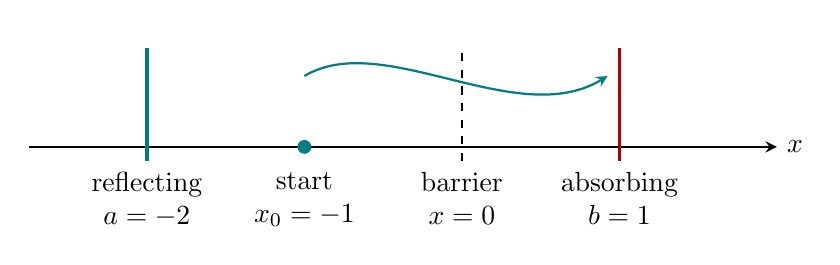
\begin{tikzpicture}[>=stealth,scale=1.0]
\draw[->,thick] (-.5,0)--(9,0) node[right] {$x$};
\draw[teal,very thick] (1,-.18)--(1,1.25); \node[align=center,below] at (1,-.2) {reflecting\\$a=-2$};
\fill[teal] (3,0) circle (2.5pt);\node[align=center,below] at (3,-.2) {start\\$x_0=-1$};
\draw[dashed,thick] (5,-.18)--(5,1.25);\node[align=center,below] at (5,-.2) {barrier\\$x=0$};
\draw[red!70!black,very thick] (7,-.18)--(7,1.25);\node[align=center,below] at (7,-.2) {absorbing\\$b=1$};
\draw[->,thick,teal] (3,.9)..controls (4,1.5) and (5.7,.2)..(6.85,.9);
\end{tikzpicture}\end{center}
\vspace{.4cm}First hit of $b$ defines the event. A first hit of the barrier is a different event and can give a different MFPT.
\end{frame}
\begin{frame}{Probability loss equals first-passage flux}
Let $p(x,t\mid x_0)$ be the \emph{killed} density on $a<x<b$, with reflecting $a$ and absorbing $b$.
\[S(t\mid x_0)=\int_a^b p(x,t\mid x_0)\,\dd x.\]
Integrating $\partial_t p=-\partial_xJ$ gives
\[\frac{\dd S}{\dd t}=J(a,t)-J(b,t)=-J(b,t).\]
For a regular boundary, the first-passage density is
$\rho_\tau(t)=-S'(t)=J(b,t)$.
\end{frame}
\begin{frame}{Survival, mean time and censoring}
Define $S(t)=\Pr(\tau_b>t)$. If the mean is finite,
\[\E[\tau_b]=\int_0^\infty S(t)\,\dd t.\]
A no-hit trajectory at observation time $T_{\mathrm{obs}}$ is right-censored.
\[\E[\min(\tau_b,T_{\mathrm{obs}})]=\int_0^{T_{\mathrm{obs}}}S(t)\,\dd t.\]
This restricted mean is not necessarily the full MFPT.
\end{frame}
\begin{frame}{Survival and a finite observation horizon}
\begin{center}
\begin{tikzpicture}\begin{axis}[width=.75\textwidth,height=4.4cm,xmin=0,xmax=8,ymin=0,ymax=1.05,axis lines=left,xlabel={$t$},ylabel={$S(t)$},xtick={0,3,8},xticklabels={$0$,$T_{\rm obs}$,$8$},ytick={0,1},samples=100,domain=0:8]
\addplot[teal,very thick]{exp(-x/4)};
\draw[red!70!black,dashed,thick] (axis cs:3,0)--(axis cs:3,.4724);
\end{axis}\end{tikzpicture}\end{center}
\vspace{-0.2cm}\small Example: $S(t)=e^{-t/4}$, shown as an illustration. The area before $T_{\rm obs}$ is a restricted mean. The unknown tail is needed for the full mean.
\end{frame}
\begin{frame}{Derive the backward MFPT equation}
Let $\tau_b$ be the first hit of $b$ and $\sigma=\min(\Delta t,\tau_b)$. The Markov property and $T(b)=0$ give the stopped first-step identity
\[T(x)=\E_x\!\left[\sigma+T(X_\sigma)\right].\]
For an interior starting point, the small-time limit, with suitable regularity, yields
\[\boxed{\mathcal LT(x)=-1,\quad T'(a)=0,\quad T(b)=0.}\]
Equivalently, apply Dynkin's formula to the stopped process. For constant $D$, $\mathcal LT=DT''-D\beta F'T'$.
\end{frame}
\begin{frame}{Integrating-factor derivation}
For an equilibrium It\^o diffusion with positive $D(x)$,
\[\mathcal LT=e^{\beta F}\frac{\dd}{\dd x}\!\left[D e^{-\beta F}T'\right]=-1.\]
Apply $T'(a)=0$, integrate from $a$ to $y$, then apply $T(b)=0$:
\[\boxed{T(x_0)=\int_{x_0}^{b}\!\dd y\,\frac{e^{\beta F(y)}}{D(y)}\int_a^y\!\dd z\,e^{-\beta F(z)}.}\]
Assumes a reflecting $a$, absorbing $b$, finite MFPT and adequate regularity.
\end{frame}

\begin{frame}{MFPT integral: intermediate steps}
Write $w(x)=e^{-\beta F(x)}$ and $I(y)=\int_a^y w(z)\,\dd z$. From $\mathcal LT=-1$,
\[\frac{\dd}{\dd x}\big[D(x)w(x)T'(x)\big]=-w(x).\]
Using $T'(a)=0$ yields $D(y)w(y)T'(y)=-I(y)$. Then
\[
T(b)-T(x_0)=\int_{x_0}^{b}T'(y)\,\dd y,
\]
and $T(b)=0$ gives the integral formula on the preceding slide.
\end{frame}
\begin{frame}{Analytic check: free diffusion}
For $F=0$ and constant $D$, the integral reduces to
\[\boxed{T(x_0)=\frac{(b-a)^2-(x_0-a)^2}{2D}.}\]
\begin{itemize}\item $T(b)=0$ and $T'(a)=0$.\item $T$ has units of time and scales as $1/D$.\item Moving either boundary changes the experiment and its answer.\end{itemize}
\end{frame}

\begin{frame}{From Fokker--Planck to a grid generator}
For spacing $h$ and $\Delta F_i=F_{i+1}-F_i$, use nearest-neighbour rates
\[
Q_{i,i+1}=\frac{D}{h^2}e^{-\beta\Delta F_i/2},\qquad
Q_{i+1,i}=\frac{D}{h^2}e^{+\beta\Delta F_i/2}.
\]
With $Q_{ii}=-\sum_{j\ne i}Q_{ij}$, row probabilities satisfy $\dot p=pQ$ and $\pi_i\propto e^{-\beta F_i}$ satisfies detailed balance: $\pi_iQ_{ij}=\pi_jQ_{ji}$. For a target removed from the transient set $S$,
\[-Q_{SS}\,\mathbf T=\mathbf 1.\]
\end{frame}
\begin{frame}{Hands-on 3: compare three routes}
\textbf{Open:} \texttt{notebooks/03\_kinetics\_investigation.ipynb}, sections 1--4.
\begin{enumerate}\item Simulate independent first-passage trajectories.\item Evaluate the backward-equation integral by quadrature.\item Solve a discrete generator equation $-Q_{SS}T=\mathbf 1$.\end{enumerate}
Match $F$, $D$, $x_0$, $a$ and $b$. Report censoring and uncertainty. Refine the time step and grid before interpreting disagreement.
\end{frame}
\begin{frame}{Why numerical comparisons can disagree}
\begin{itemize}\item \textbf{Sampling:} finitely many independent trajectories.\item \textbf{Time step:} endpoint detection can miss crossings.\item \textbf{Grid spacing:} the finite-state model approaches the continuum on refinement.\item \textbf{Censoring:} paths not arriving before the horizon have unknown full times.\end{itemize}
For the default teaching model, quadrature gives approximately $5.13$ in dimensionless time units.
\end{frame}

\begin{frame}{Exercise: make convergence measurable}
\small
\begin{center}
\begin{tabular}{lcccc}
\hline
Run & $\Delta t$ & $N$ & censored fraction & restricted mean $\pm$ SE\\
\hline
1 & $\Delta t$ & $N$ & \rule{1cm}{.1pt} & \rule{1.7cm}{.1pt}\\[3pt]
2 & $\Delta t/2$ & $N$ & \rule{1cm}{.1pt} & \rule{1.7cm}{.1pt}\\[3pt]
3 & $\Delta t/4$ & $N$ & \rule{1cm}{.1pt} & \rule{1.7cm}{.1pt}\\
\hline
\end{tabular}\end{center}
For independent paths, compute SE from the sample SD of $\min(\tau,T_{\rm obs})$ divided by $\sqrt N$. Compare with quadrature ($\approx5.13$) only when censoring is negligible. Vary $N$ and grid spacing separately.
\end{frame}
\begin{frame}{MFPT versus a phenomenological rate}
\begin{itemize}
\item $T(x)$ refers to a specific initial point and stopping event. For initial density $\rho_0$, $\langle\tau\rangle_{\rho_0}=\int T(x)\rho_0(x)\,\dd x$.
\item $1/\langle\tau\rangle$ is the reciprocal mean of that experiment.
\item A two-state rate interpretation requires suitable basin definitions and a separation between intrabasin relaxation and escape.
\item A boundary at the barrier and a boundary in the product well have different recrossing behavior.
\end{itemize}
\end{frame}
\begin{frame}{Starting ensembles and escape rates}
Starting at a point, drawing from equilibrium restricted to $A$, or drawing from a quasi-stationary distribution defines different experiments.
\begin{itemize}
\item Within a metastable basin, relaxation can precede rare escape.
\item A quasi-stationary initial distribution gives exponential survival in its domain, under the usual killed-process conditions.
\item More generally, an approximately exponential tail $S(t)\simeq A e^{-kt}$ can support an escape-rate interpretation after initial transients.
\end{itemize}
\small The fitted $k$ and reciprocal full MFPT need not agree for arbitrary preparations.
\end{frame}
\begin{frame}{Optional: the committor}
For reactant $A$ and product $B$, the forward committor is
\[q(x)=\Pr_x(\tau_B<\tau_A),\qquad \mathcal Lq=0.\]
Boundary conditions: $q(a)=0$, $q(b)=1$. For variable $D$ in equilibrium,
\[q(x)=\frac{\int_a^x e^{\beta F(y)}/D(y)\,\dd y}{\int_a^b e^{\beta F(y)}/D(y)\,\dd y}.\]
MFPT asks \emph{how long}; the committor asks \emph{which state first}.
\end{frame}
\begin{frame}{From the toy model to molecules}
For a collective variable $s(\mathbf R)$, define the equilibrium marginal and free energy
\[p_{\rm eq}(s)=\int \dd\mathbf R\,\rho_{\rm eq}(\mathbf R)\delta[s-s(\mathbf R)],\quad F(s)=-k_BT\ln p_{\rm eq}(s)+C.\]
Before predicting kinetics, ask:
\begin{enumerate}\item Do $A$ and $B$ represent the desired molecular event?\item Is the projected dynamics approximately Markovian?\item Is $D(s)$ known, with units and uncertainty?\item Are predictions robust to boundaries and hidden slow coordinates?\end{enumerate}
\end{frame}

\begin{frame}{A molecular projection can hide slow variables}
\begin{center}
\begin{tikzpicture}[>=stealth]
\draw[->] (0,0)--(8,0) node[right] {coordinate $s$};
\draw[->] (0,0)--(0,3.2) node[above] {hidden coordinate $z$};
\fill[teal] (3,0.9) circle (3pt);\fill[orange!90!black] (3,2.4) circle (3pt);
\draw[dashed] (3,0)--(3,3);\node[teal,right] at (3.2,.9) {configuration 1};
\node[orange!90!black,right] at (3.2,2.4) {configuration 2};
\end{tikzpicture}\end{center}
\small Both configurations have the same $s$ but may have different committors. A one-dimensional Markov model then loses information about future behavior.
\end{frame}
\begin{frame}{Changing coordinates: density and diffusion}
Let $y=g(x)$ be a smooth monotone map. Probability conservation gives
\[p_y(y)=p_x(x)\left|\frac{\dd x}{\dd y}\right|,\qquad
D_y(y)=[g'(x)]^2D_x(x).\]
Thus $F_y(y)=F_x(x)+k_BT\ln|g'(x)|+C$ for these coordinate densities.
\begin{itemize}
\item Free-energy profiles and diffusivities depend on the coordinate.
\item If transformed consistently, a physical first-passage event is invariant.
\item Projecting many molecular coordinates into one is a separate approximation and can create memory.
\end{itemize}
\end{frame}
\begin{frame}{Take-home questions}
\begin{enumerate}\item Can two models have the same equilibrium density and different MFPTs?\item What do reflecting and absorbing boundaries encode?\item Why can a finite simulation underestimate a full passage time?\item When is a one-dimensional molecular diffusion model plausible?\end{enumerate}
Read \texttt{notes/00\_foundations.md} and \texttt{notes/derivations.md} for full derivations.
\end{frame}
\begin{frame}{References and teaching material}
\footnotesize
\begin{itemize}
\item C. W. Gardiner, \emph{Handbook of Stochastic Methods}, 3rd ed., Springer (2004).
\item P. H\"anggi, P. Talkner, M. Borkovec, Rev. Mod. Phys. \textbf{62}, 251 (1990), \href{https://doi.org/10.1103/RevModPhys.62.251}{doi:10.1103/RevModPhys.62.251}.
\item G. Hummer, New J. Phys. \textbf{7}, 34 (2005), \href{https://doi.org/10.1088/1367-2630/7/1/034}{doi:10.1088/1367-2630/7/1/034}.
\item W. E and E. Vanden-Eijnden, J. Stat. Phys. \textbf{123}, 503 (2006), \href{https://doi.org/10.1007/s10955-005-9003-9}{doi:10.1007/s10955-005-9003-9}.
\item Inspired by Luca Sagresti's \href{https://github.com/lianctrl/HandsOnSession_CMLS}{HandsOnSession\_CMLS}.
\end{itemize}
\end{frame}
\end{document}
